\section{Charged-Current Inclusive Electron Neutrino Selection}
\label{sec:datamc:nueccinclusive}
This section includes supplementary material for the $\nu_e$ CC inclusive selection, expanding on \cref{sec:nueselection:inclusive}. A more complete set of plots can be found in DocDB 30694.

The outcome of the training process -- the BDT response -- and validation is given in \cref{fig:nuecc:train_e,fig:nuecc:train_d,fig:nuecc:train_event}. The different panels in the figure from left to right:
\begin{itemize}
\item The score of the BDT for the test fraction of the simulated events, divided in signal and background using truth labelling. 
\item The ROC curve. This metric shows the trade-off between a low false positive rate and a low false negative rate. Each point along the curve corresponds to a certain threshold on the score. The comparison between the test and training set is made, the smaller this difference, the lower the over fitting. The area under the ROC curve is a widely accepted metric for the performance of the classifier. 
\item The binary logistic loss of the classifier on both the training and the test set. The number of epochs is chosen such that the test data has reached an optimal value and stays stable. A large separation between the test and the training loss, or an upwards tendency of the test loss are indications of over-fitting.
\item The accuracy as a function of the tree depth. The accuracy is the fraction of correct predictions at a score threshold of $0.5$. The three depth is optimised based on the validation curve to minimise over-fitting while maintaining a high accuracy. 
\end{itemize} 

\begin{figure}[htb]
\centering
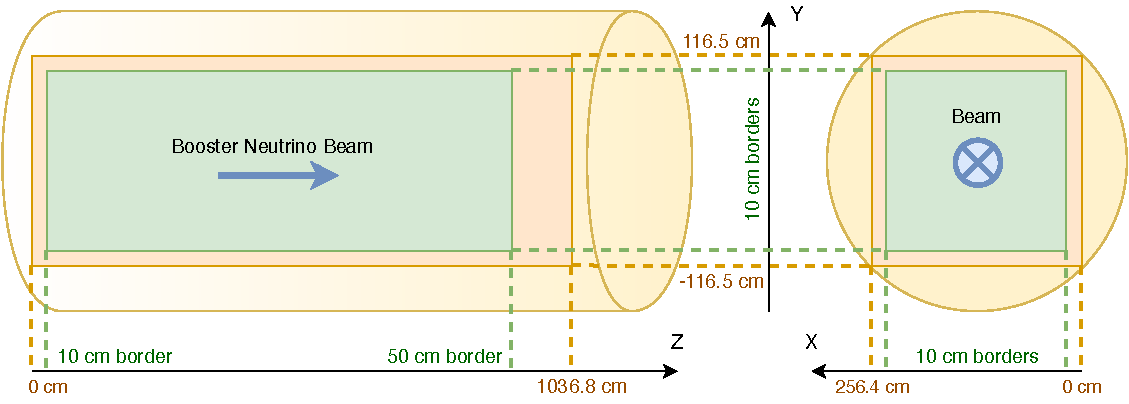
\includegraphics[width = 0.85\textwidth]{NueCCsel/Images/FidVolume.pdf}
\caption{Fiducial volume used for both the \nuecc signal definition and the \nuecc selection. The yellow cylinder represents the cryostat, the orange structure is the TPC and the green area is the fiducial volume. Both the $YZ$ (left) and $XY$ (right) projections are shown.}
\label{fig:nuecc:fidvol}
\end{figure}

\begin{figure}[htb]
\begin{center}
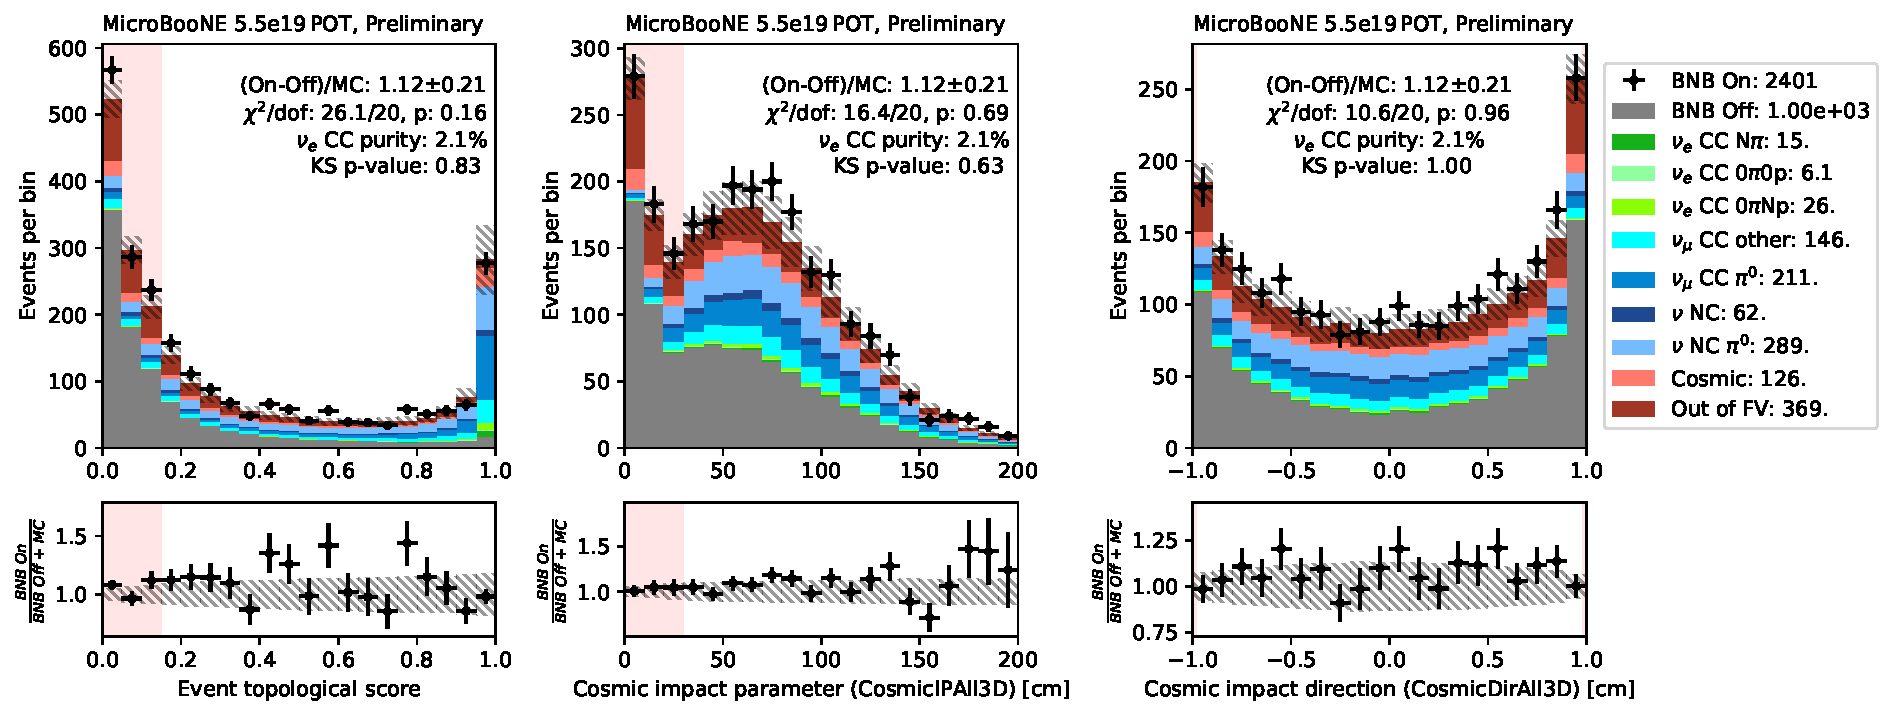
\includegraphics[height=0.27\textheight]{NueCCsel/Images/datamc/presel_1.pdf}
\caption{Data/MC comparisons for three variables used in the \nuecc preselection, \cref{sc:nuecc:presel}: the event topological score as described in \cref{sec:sliceID} and DocDB 14175 (left), The cosmic impact parameter (middle), and the cosmic impact direction (right). Events in the shaded red region are rejected. At this stage, the signal \nuecc events (green) only make up \pct{2.1} of the histogram.}
\label{fig:nuecc:presel_1}
\end{center}
\end{figure}


\begin{figure}[htb]
\begin{center}
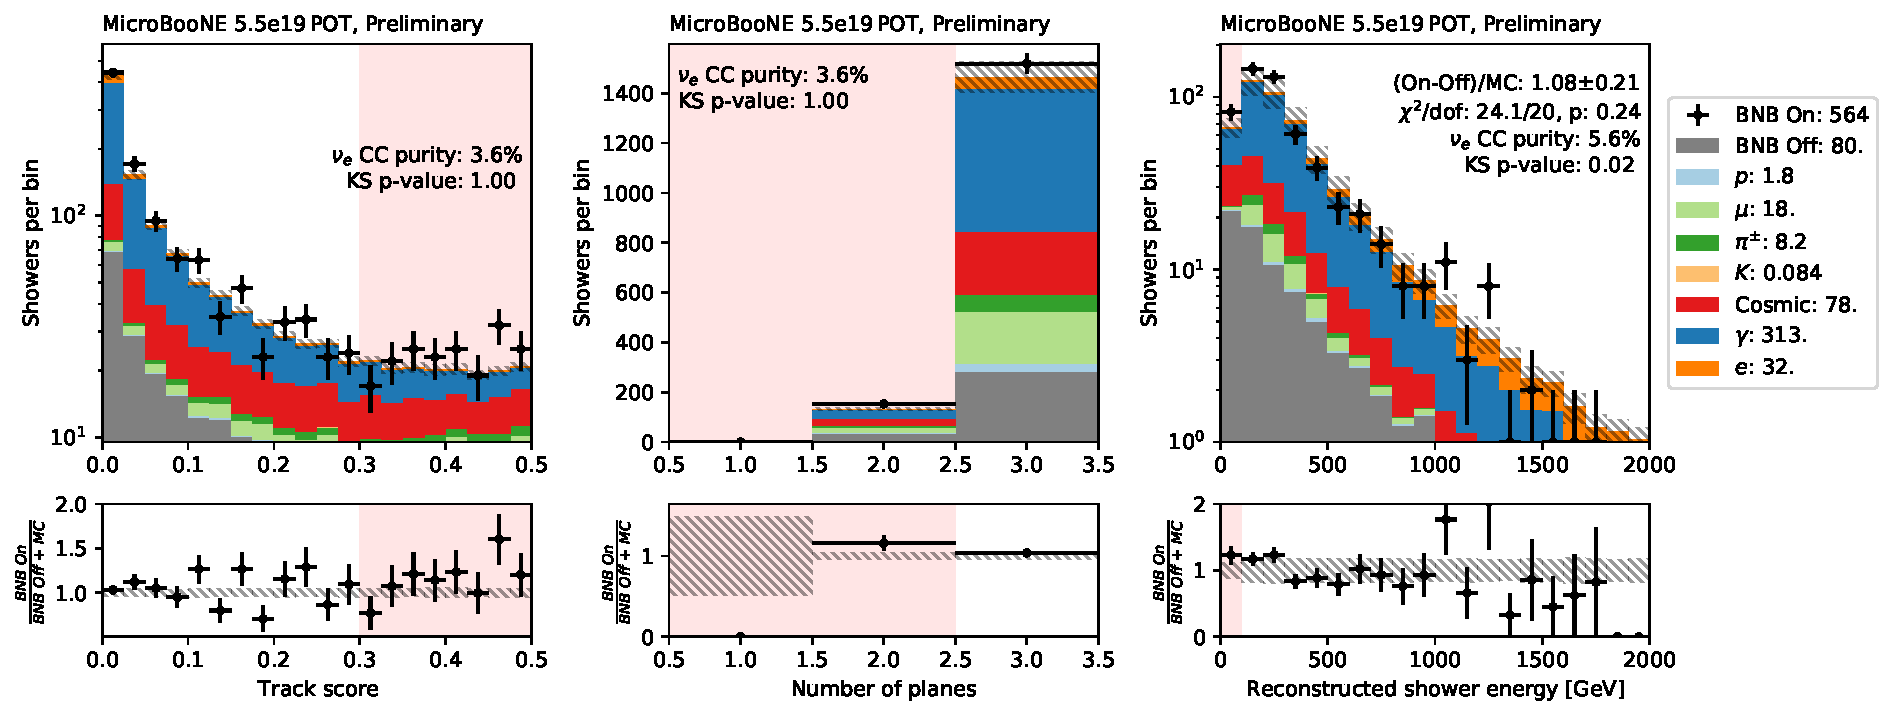
\includegraphics[height=0.27\textheight]{NueCCsel/Images/datamc/presel_2.pdf}
\caption{Data/MC comparisons used in the preselection to identify the electron neutrino candidate. From left to right, the track score, the number of planes and the reconstructed shower energy are given. Events in the shaded red region are rejected.}
\label{fig:nuecc:presel_2}
\end{center}
\end{figure}

\begin{table}[htb]
\caption{\label{tab:nuecc:e_bdt} Input variables used for electron identification by the BDT introduced in \cref{sc:nuecc:e_pid}. The data/MC distributions corresponding to the variables listed is given in \cref{fig:e_cand_1,fig:nuecc:e_cand_all}. The correlation between the variables is shown in \cref{fig:nuecc:corr_electrons}.}
\centering
\setlength{\tabcolsep}{10pt}
\renewcommand{\arraystretch}{1.25}
\begin{tabular}{| c | c |} 
\hline
Variable goal & Variable definition \\
\hline\hline
\multirow{2}{*}{$e/\gamma$ separation} & Shower vertex distance \\
                                       & \makecell{Shower \dedx at the start of the shower: \\
                                           \tabitem Collection plane, the first \SI{4}{\cm}.\\
                                           \tabitem Collection plane, the first \SI{2}{\cm}.\\
                                           \tabitem Collection plane from \SIrange{1}{4}{\cm}.\\
                                          \tabitem Three plane hit weighted mean, first \SI{4}{\cm}.
                                            }\\
\hline

\multirow{3}{*}{$\mu$-rejection} & Number of subclusters \\
                                 & Moliere angle \\
                                 & Hit fraction in the shower trunk \\
 \hline
 \multirow{1}{*}{$\pi^0$ tagging} & \textit{Second shower} number of hits \\
 \hline
 \end{tabular}
\end{table}

\begin{figure}[htb]
\centering
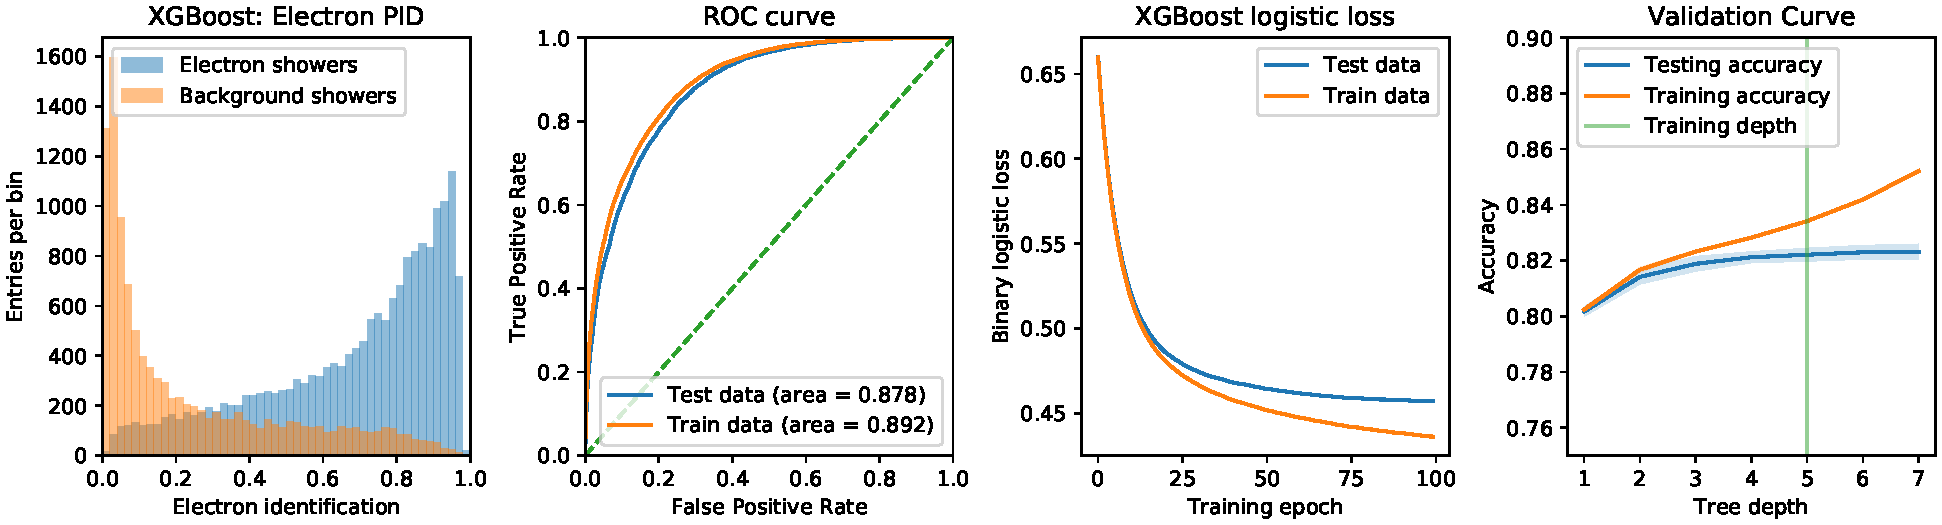
\includegraphics[width=1.0\textwidth]{NueCCsel/Images/training/e_bdt_test}
\caption[Evaluation of training performance for electron shower identification]{Evaluation of training performance for electron shower identification. Different panels explained in the text.}
\label{fig:nuecc:train_e}
\end{figure}

\begin{figure}[htb] 
\begin{center}
    \begin{subfigure}{\textwidth}
    \centering
    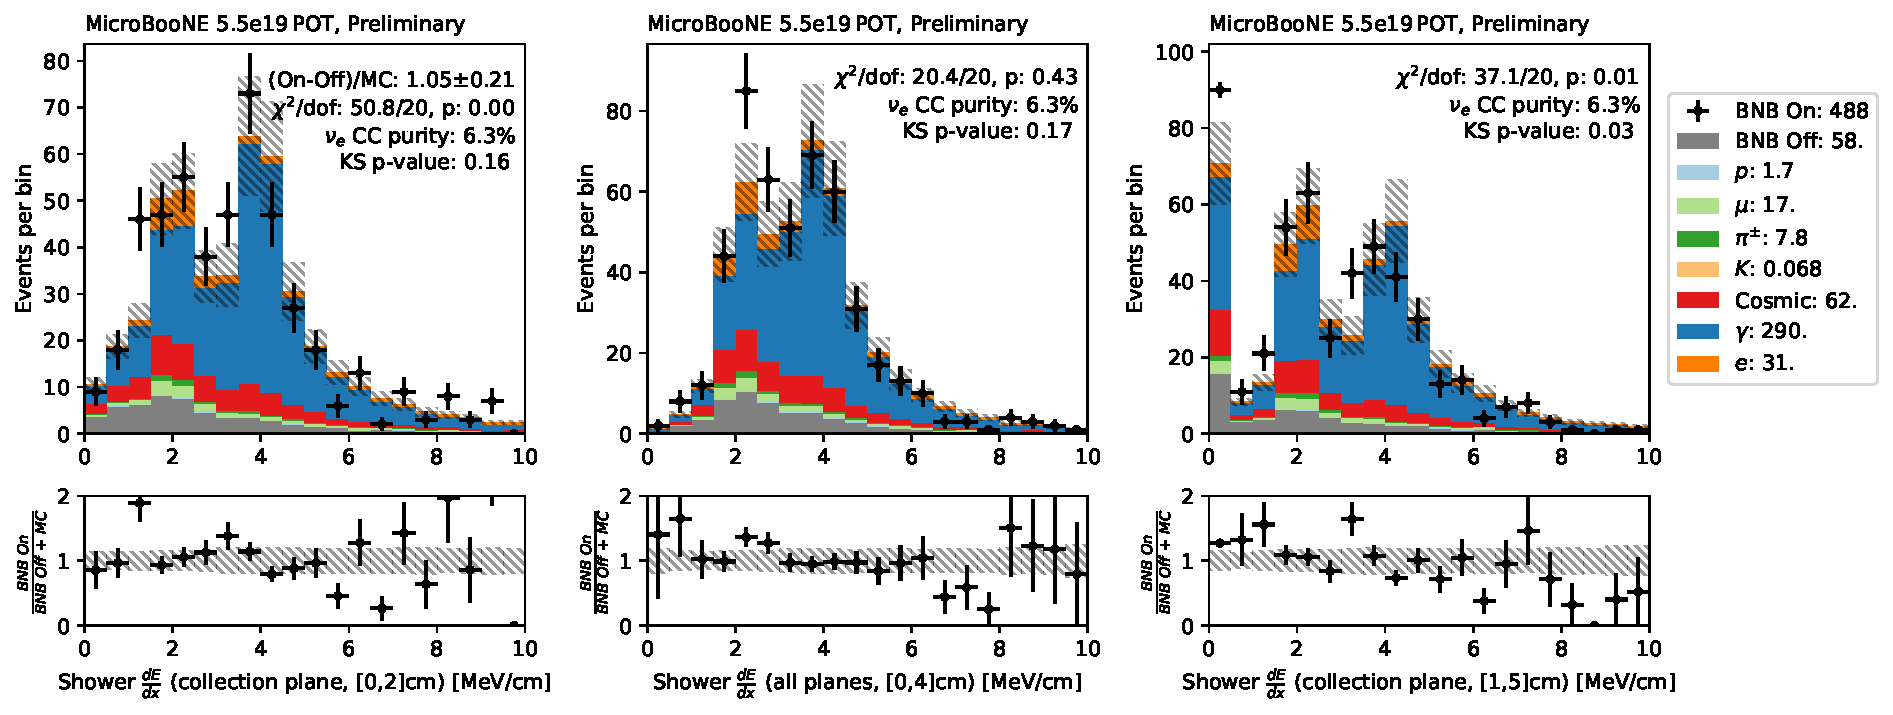
\includegraphics[height=0.27\textheight]{NueCCsel/Images/datamc/e_cand_dedx}
    \caption{\label{fig:nuecc:e_cand_dedx} Three variables used to characterise the \dedx at the start of the electron candidate shower.}
    \end{subfigure}
    \begin{subfigure}{\textwidth}
    \centering
    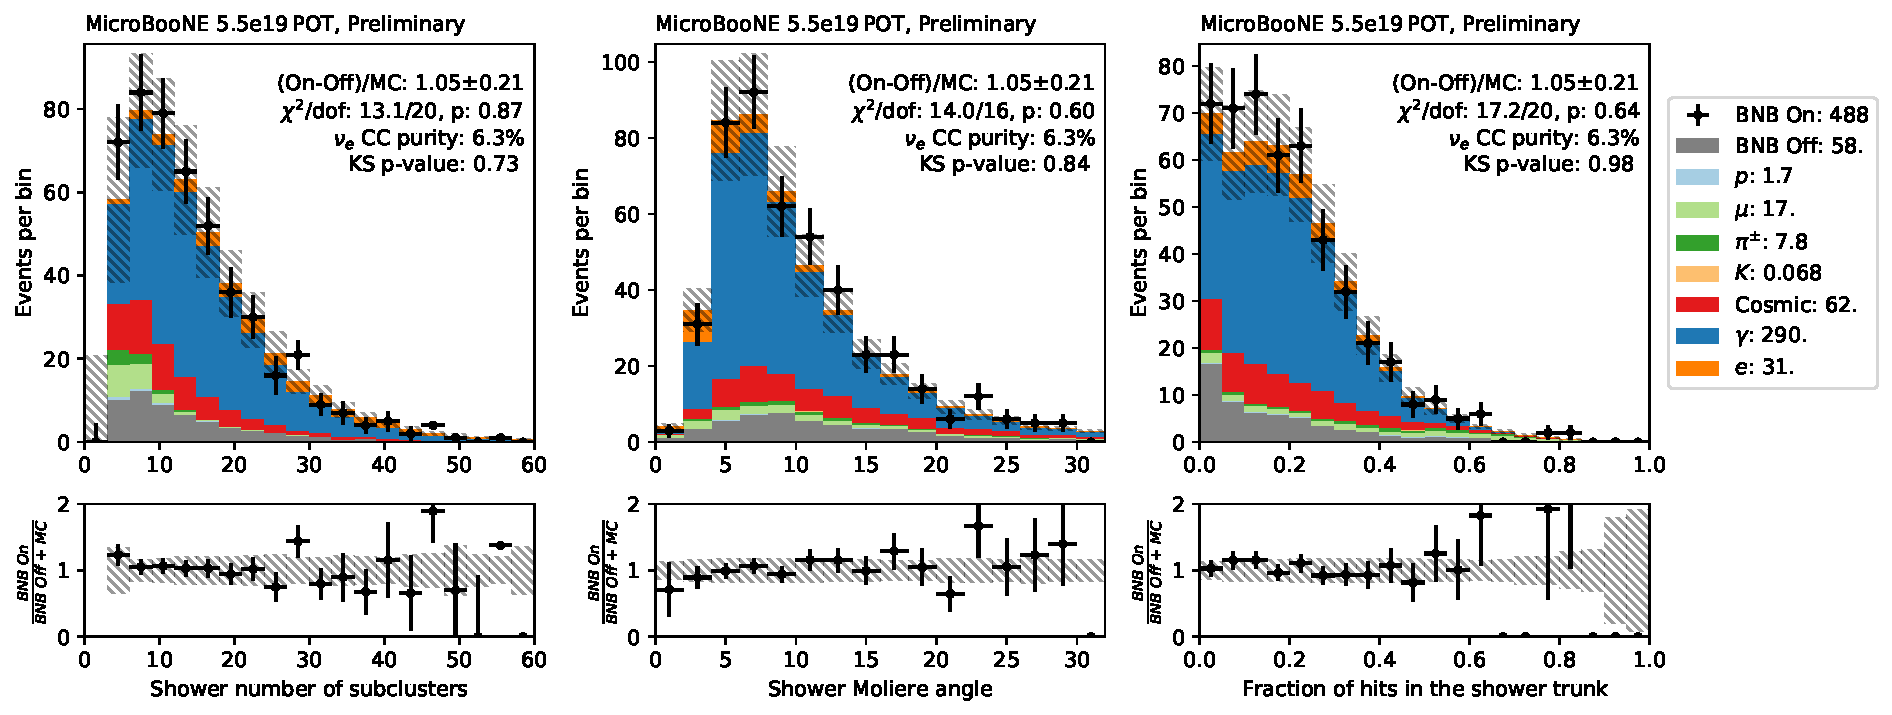
\includegraphics[height=0.27\textheight]{NueCCsel/Images/datamc/e_cand_2.pdf}
    \caption{\label{fig:nuecc:e_cand2} Geometrical properties of the electron candidate shower.}
    \end{subfigure}
    \begin{subfigure}{\textwidth}
    \centering
    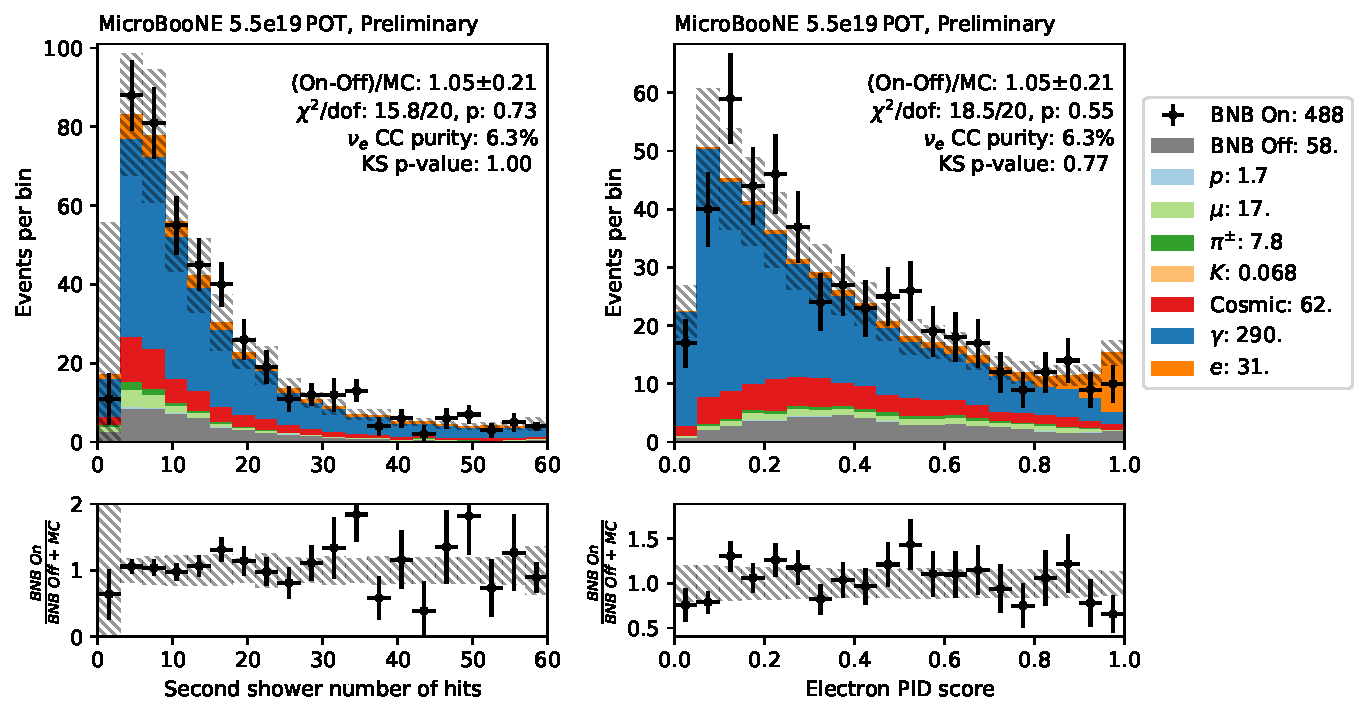
\includegraphics[height=0.27\textheight]{NueCCsel/Images/datamc/e_cand_3.pdf}
    \caption{\label{fig:nuecc:e_cand3} The number of hits in the second shower tagging (left) and the electron PID score obtained from the BDT (right).}
    \end{subfigure}
    \end{center}
\caption{\label{fig:nuecc:e_cand_all} Data/MC comparisons for the input variables of the electron shower classifier, as listed in \cref{tab:nuecc:e_bdt} and its response (bottom right panel). The two input variables with the strongest separation are shown in the main section, see \cref{fig:e_cand_1}.}
\end{figure}

\begin{figure}[htb]
\centering
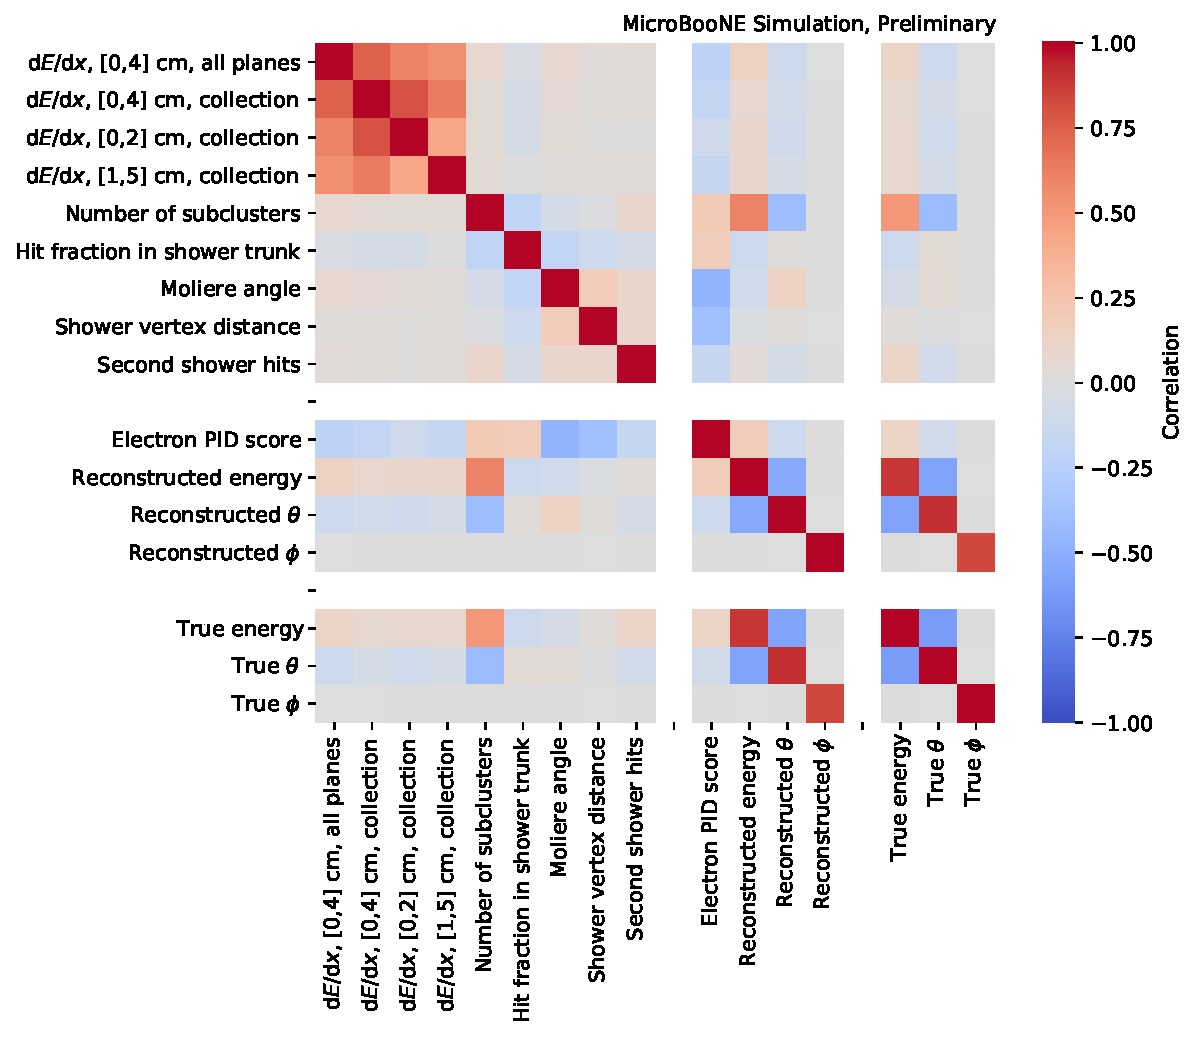
\includegraphics[width=0.7\textwidth]{NueCCsel/Images/truth/e_cand_corr.pdf}
\caption[Correlation matrix of the variables of interest in the electron identification step]{Correlation matrix of the variables of interest in the electron identification step. The first group (top-left) contains the variables used in the electron PID. The second group (middle) are the BDT score and the reconstructed lepton kinematics that can be compared with their simulated counterparts in the third group (bottom-left).}
\label{fig:nuecc:corr_electrons}
\end{figure}

\clearpage
\begin{table}[htb]
\caption{\label{tab:nuecc:d_bdt} Input variables used for other daughter identification by the BDT. The data/MC distributions corresponding to the variables listed is given in \cref{fig:nuecc:other_cand1,fig:nuecc:other_cand2}.}
\centering
\setlength{\tabcolsep}{10pt}
\renewcommand{\arraystretch}{1.25}
\begin{tabular}{|c|c|}
\hline
Variable goal                            & Variable definition             \\ \hline \hline
\multirow{3}{*}{$\mu$-rejection}         & Track log likelihood PID    \\ 
                                         & Calorimetric / range-based energy under proton hypothesis \\
                                         & MCS / range-based momentum under muon hypothesis \\
\hline
\multirow{3}{*}{$\gamma$-identification} & Vertex distance            \\
                                    & Angle w.r.t. the electron shower \\
                                    & Track score                \\ \hline
\multirow{3}{*}{Particle hierarchy} & Daughter generation        \\
                                    & Has a shower-like daughter \\
                                    & Has a track-like daughter  \\ \hline
\end{tabular}
\end{table}

\begin{figure}
\centering
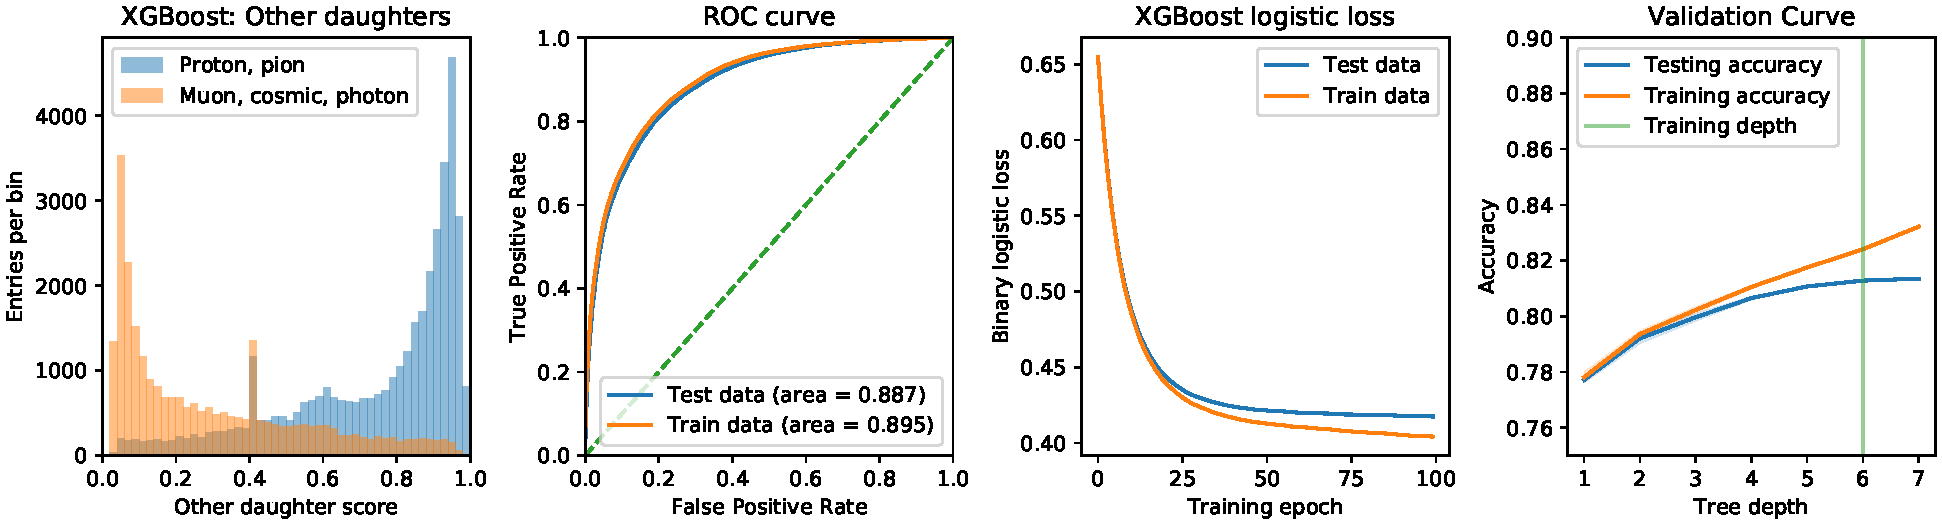
\includegraphics[width=\textwidth]{NueCCsel/Images/training/daughter_bdt_test}
\caption[Evaluation of training performance for the other daughters in the event]{Evaluation of training performance for the \textit{other daughters} in the event.}
\label{fig:nuecc:train_d}
\end{figure}

\begin{figure}[htb] 
\begin{center}
    \begin{subfigure}{\textwidth}
    \centering
    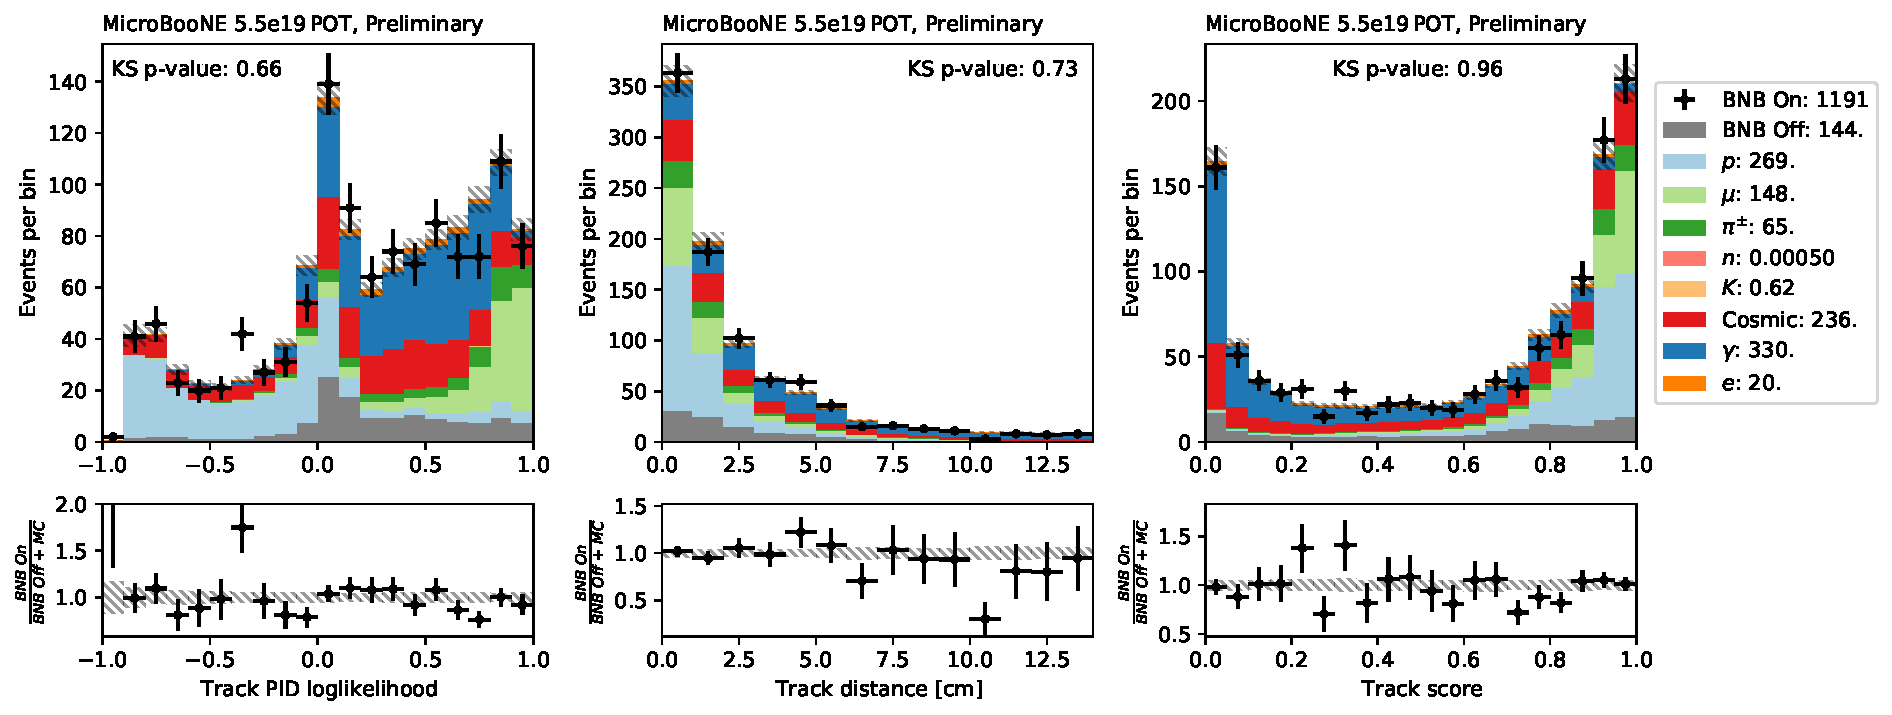
\includegraphics[height=0.27\textheight]{NueCCsel/Images/datamc/pre_daughter_1}
    \caption{\label{fig:nuecc:other_cand1} Track related variables: PID log likelihood, vertex distance and track score.}
    \end{subfigure}
    \begin{subfigure}{\textwidth}
    \centering
    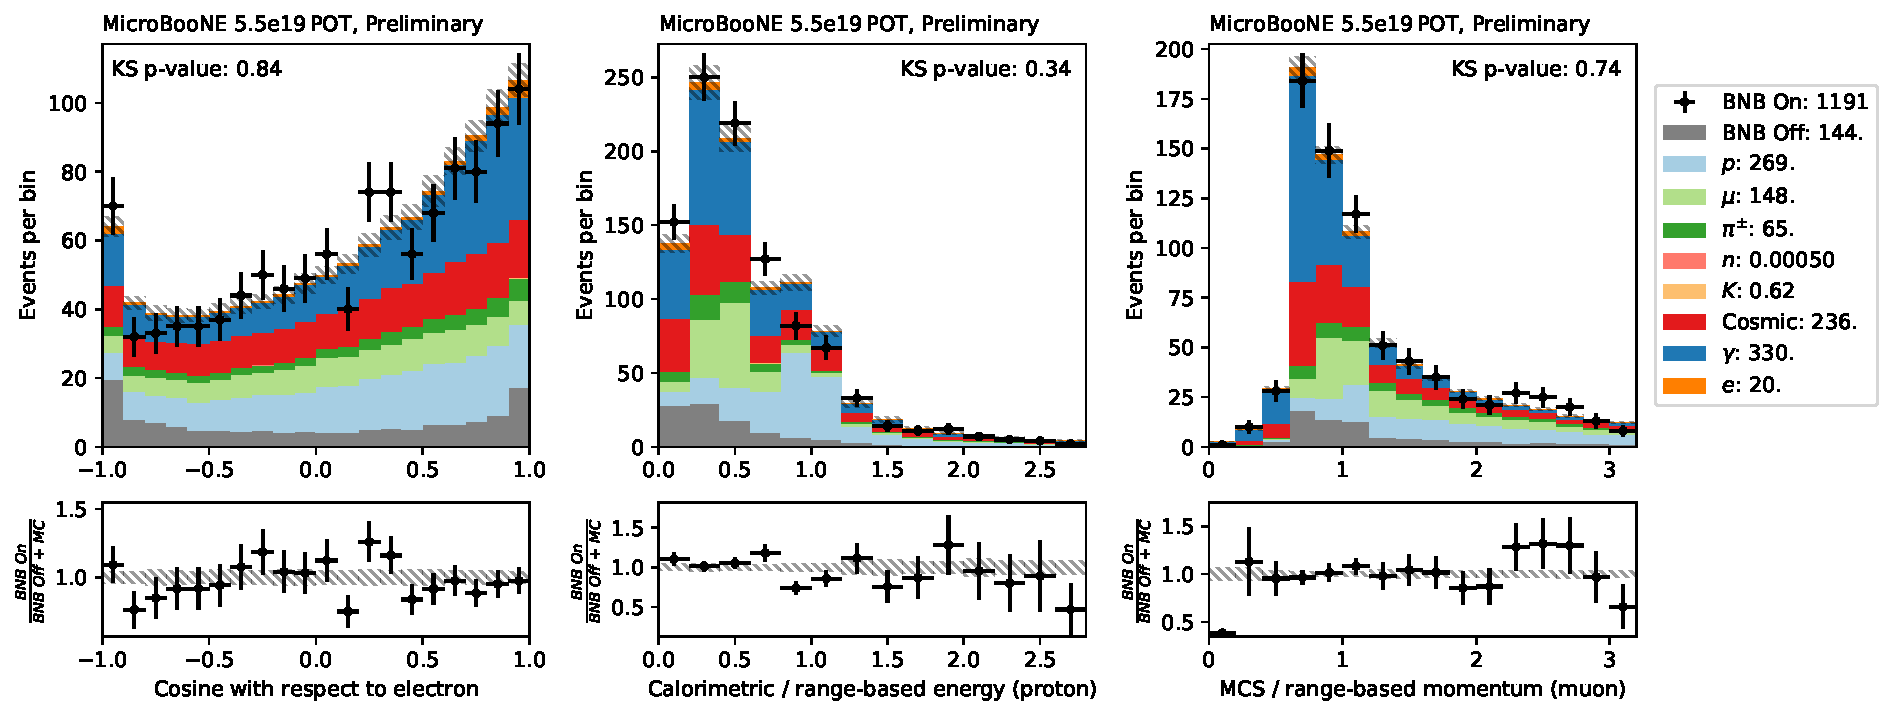
\includegraphics[height=0.27\textheight]{NueCCsel/Images/datamc/pre_daughter_2}
    \caption{\label{fig:nuecc:other_cand2} The angle of a reconstructed particle and the candidate electron shower (right), and the proton (middle) and (muon) consistency variables.}
    \end{subfigure}
    \begin{subfigure}{\textwidth}
    \centering
    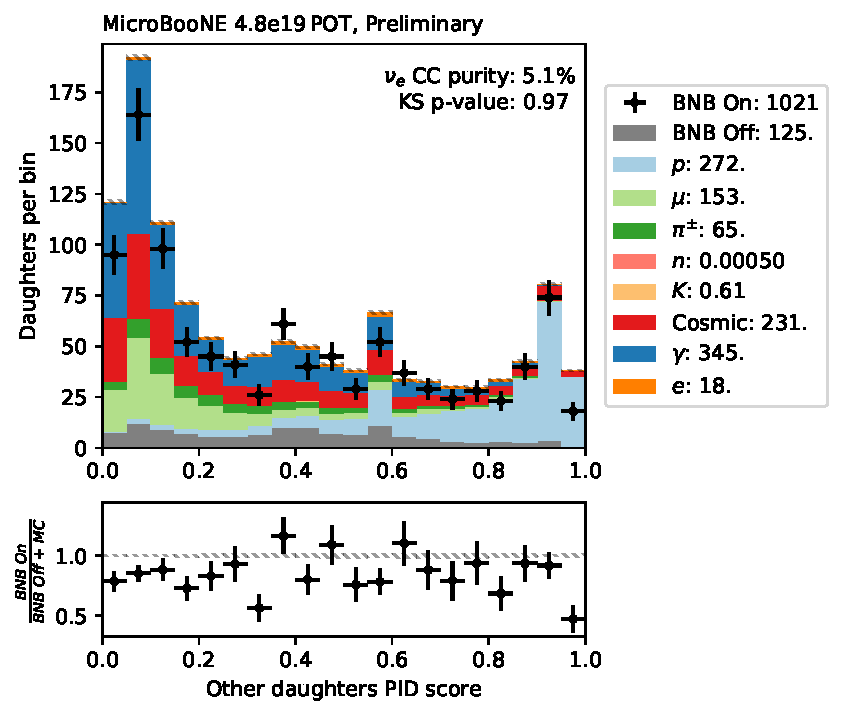
\includegraphics[height=0.27\textheight]{NueCCsel/Images/datamc/daughters_bdt.pdf}
    \caption{\label{fig:nuecc:other_result} Response of the classifier for all other daughters in the preselected events.}
    \end{subfigure}
    \end{center}
\caption{\label{fig:nuecc:other_cand_all} Data/MC comparisons for the six most important input variables of the \textit{other daughters} classifier. The bottom row shows the response of the BDT}
\end{figure}

\clearpage

\begin{figure}[t]
\centering
\begin{subfigure}{\textwidth}
    \centering
    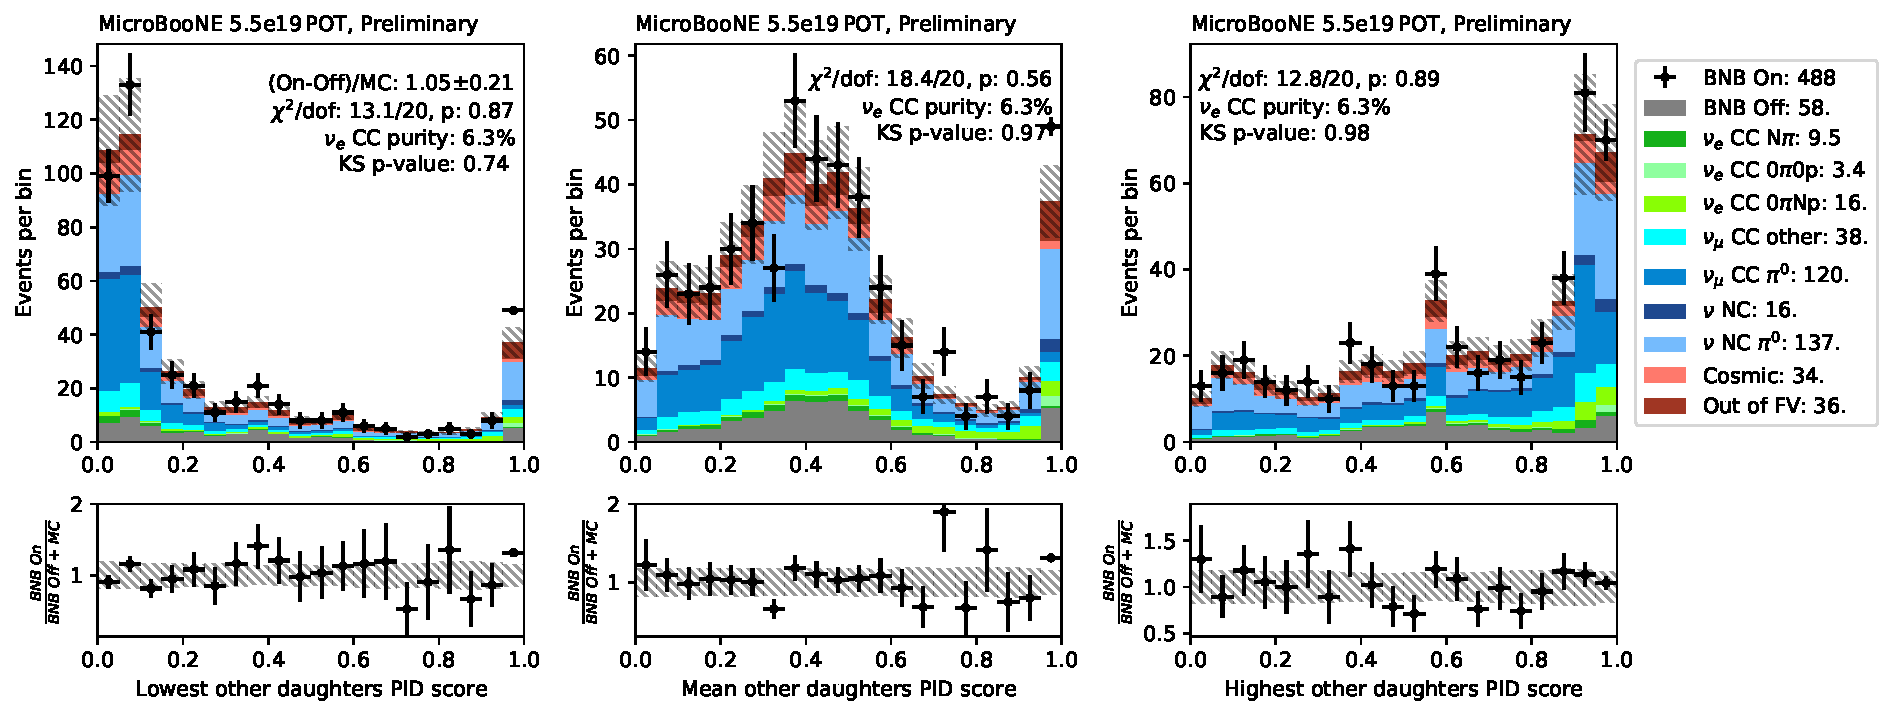
\includegraphics[height=0.27\textheight]{NueCCsel/Images/datamc/event_bdt_input_1.pdf}
    \caption{Three aggregation variables deduced from the other daughters BDT: the minimum (left), average (middle) and maximum (right).}
    \label{fig:nuecc:bdt_event_input1}
    \end{subfigure}
    \begin{subfigure}{\textwidth}
    \centering
    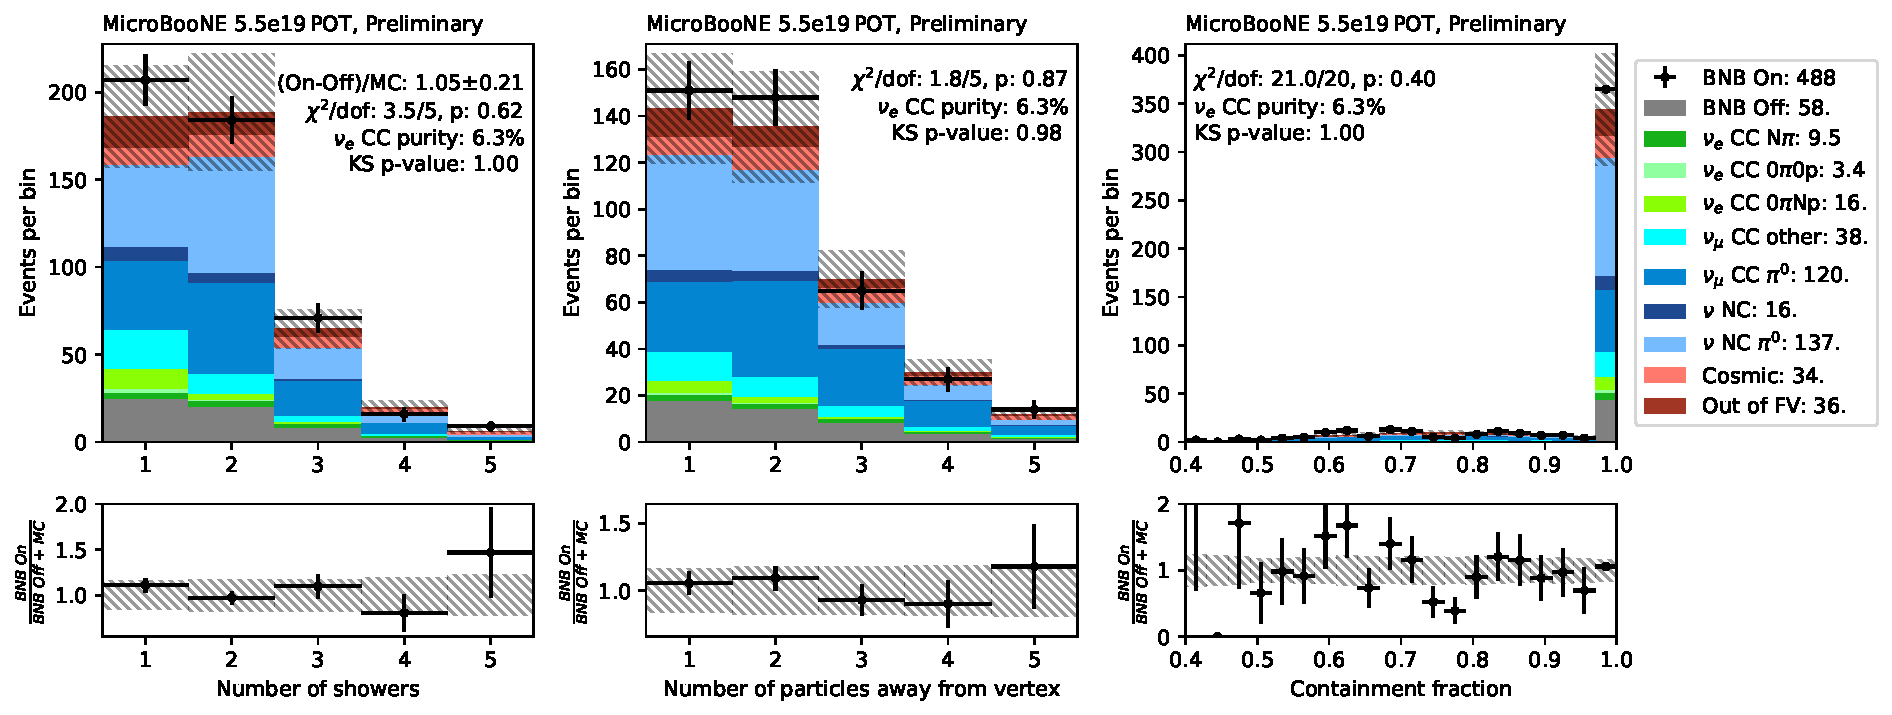
\includegraphics[height=0.27\textheight]{NueCCsel/Images/datamc/event_bdt_input_2.pdf}
    \caption{Topological variables characterising the event: number of showers (left), number of particles that is not attached to the vertex (middle) and containment (right).}
    \label{fig:nuecc:bdt_event_input2}
    \end{subfigure}
\caption[Variables used for the final \nuecc event selection classifier]{Six of the seven variables used for the final \nuecc event classifier. The most important variable is the electron PID score which is shown in the right panel of \cref{fig:nuecc:e_cand3}.}
\label{fig:nuecc:bdt_event_input}
\end{figure}

\begin{figure}[b]
\centering
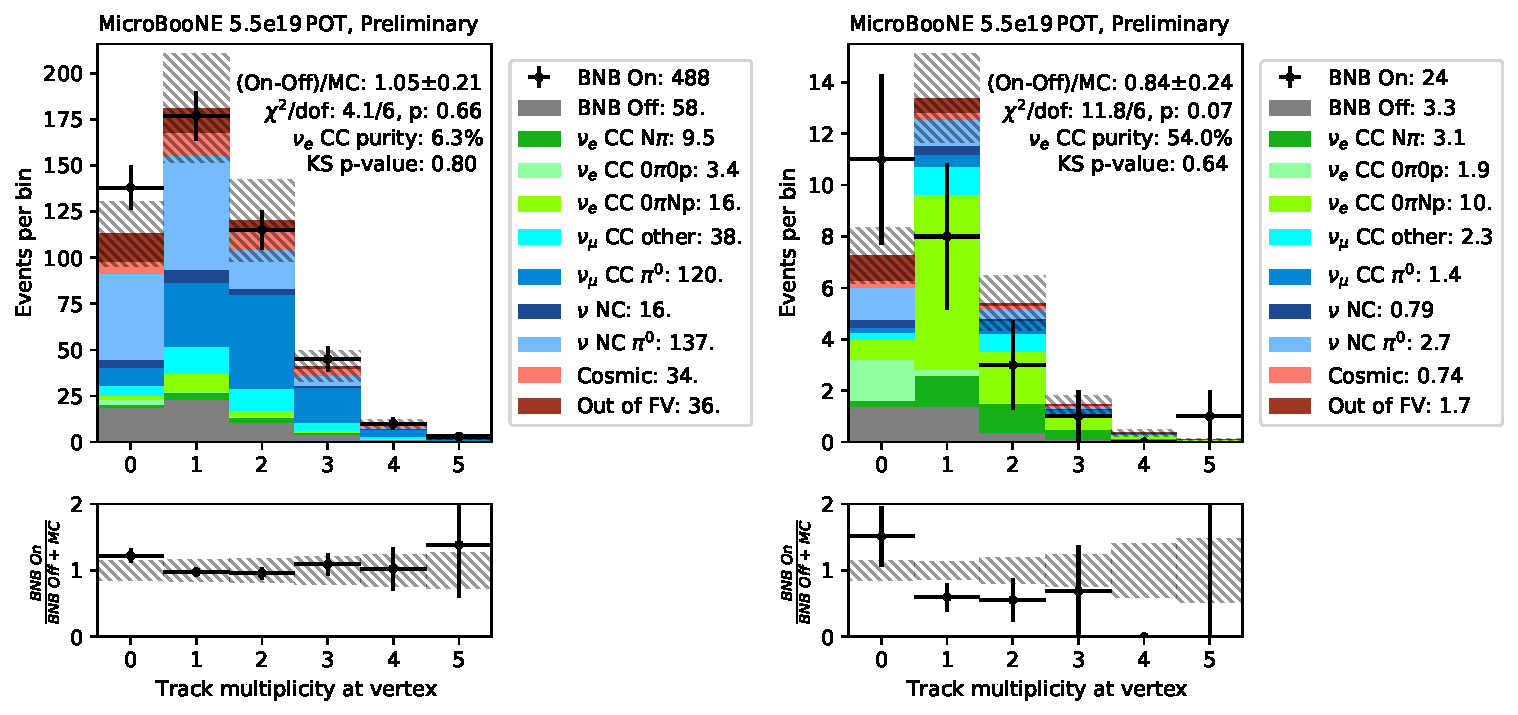
\includegraphics[height=0.27\textheight]{NueCCsel/Images/datamc/event_trk_at_vtx.pdf}
\caption[Vertex track multiplicity]{Track multiplicity near the vertex (start point within \SI{3}{\cm}) after the preselection (left) and the full \nuecc selection (right).}
\label{fig:nuecc:trk_at_vtx}
\end{figure}

\begin{figure}[htb]
\centering
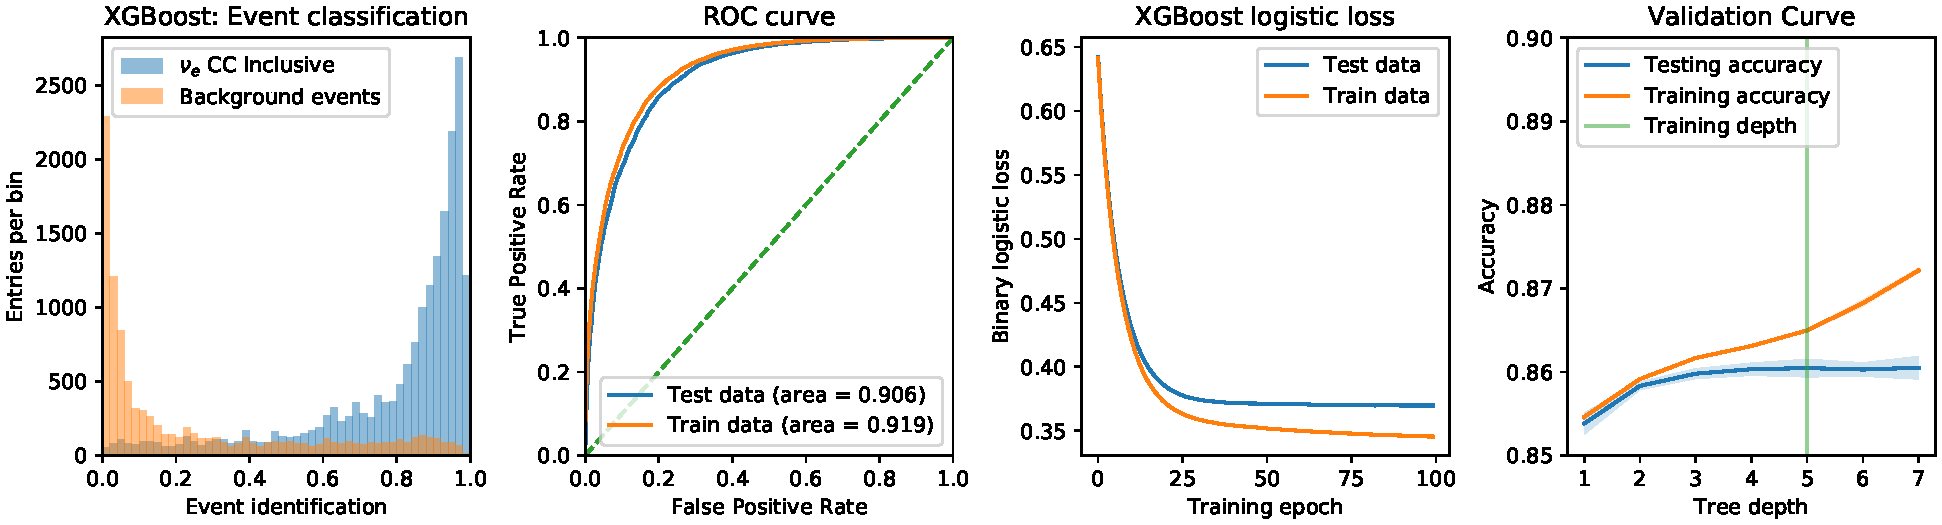
\includegraphics[width=\textwidth]{NueCCsel/Images/training/event_bdt_test.pdf}
\caption[Evaluation of training performance for the \nuecc event classification]{Evaluation of training performance for the \nuecc event classification.}
\label{fig:nuecc:train_event}
\end{figure}

\begin{figure}[htb]
    \centering
    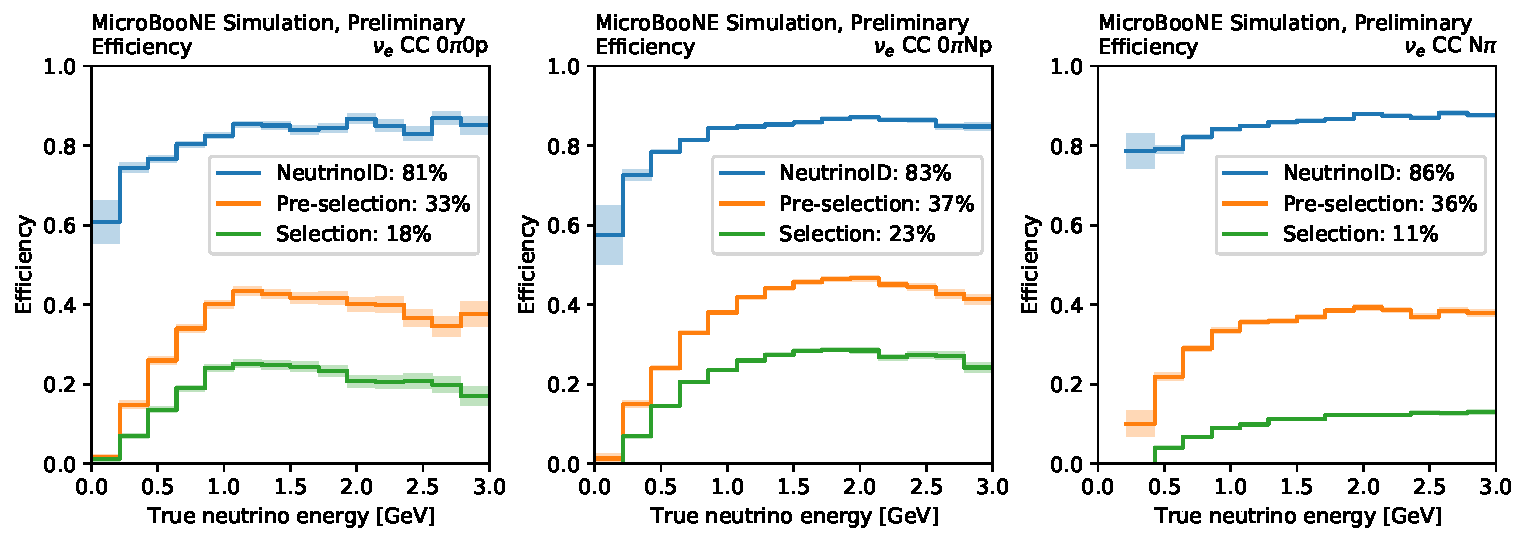
\includegraphics[width=\textwidth]{NueCCsel/Images/truth/efficiency_cat_2.pdf}
    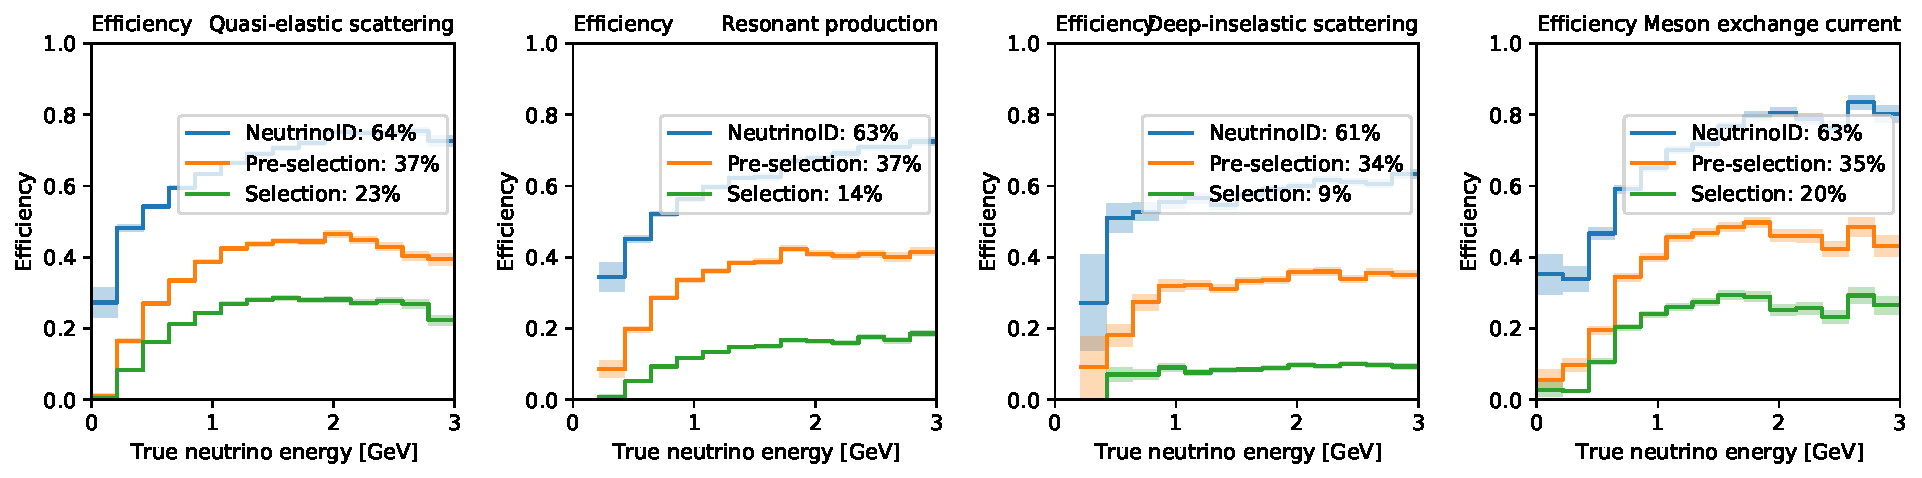
\includegraphics[width=\textwidth]{NueCCsel/Images/truth/efficiency_int.pdf}
    \caption[Efficiency of the different stages in the \nuecc selection in function of the true neutrino energy]{Efficiency of the different stages in the \nuecc selection in function of the true neutrino energy. The three panels in the top row correspond to different final state topologies, the panels in the bottom row show the efficiency for different interaction modes. The uncertainties on the integrated efficiency in the legend is $\order{\pct{0.1}}$ for all cases.}
    \label{fig:nuecc:eff}
\end{figure}